\chapter{Estado del arte}

\noindent\fbox{
	\parbox{\textwidth}{
		En este capítulo se analizará más a fondo la situación del problema, las soluciones ya realizadas, las herramientas que se pueden utilizar para realizar la solución, desde un punto de vista crítico.
	}
}

\section{Asistentes de Voz: Escuchar, procesar, responder}

Los Asistentes de Voz podrían definirse como un agente software que puede interpretar el habla humana y responder usando una voz sintetizada, según Matthew Hoy en su introducción a los Asistentes de Voz \cite{vaintroduction-matthewhoy}. 

En general, esperan a ser invocados por una palabra clave, tras lo cual graban lo que se dice y lo procesa, interpretándolo como un comando. Ese comando puede implicar desde responder con la información necesaria, pasando por interactuar con el dispositivo donde está instalado (por poner un ejemplo, pidiendo controlar elementos multimedia), hasta poder incluso manejarse con otros dispositivos dentro o fuera de su alcance.

\subsection{Una reseña histórica}
La historia de los Asistentes de este tipo está ligada como la aplicación de dos grandes campos de la Inteligencia Artificial: el Reconocimiento de Voz y la Síntesis de Voz.
\begin{itemize}
	\item El \textbf{Reconocimiento de Voz} persigue la conversión de una grabación de una voz a un texto con el mismo mensaje que el hablado
	\item La \textbf{Síntesis de Voz} busca justamente lo contrario: A través de un texto, lograr que una voz lo comunique.
\end{itemize}

Igualmente, profundizaremos en estos dos conceptos en sus secciones correspondientes, un poco más adelante.

En esta reseña histórica veremos los pasos relevantes en ambos campos hasta el primer Asistente de Voz.

\subsubsection{Experimentando con la voz}
Si bien la historia del reconocimiento de voz es más reciente, hace dos siglos se trataba de modelar el lenguaje según el movimiento del tracto vocal, dando así un paso en su síntesis.

La primera instancia de aparatos que usen la voz data de un juguete de 1918 denominado Radio Rex, el cual al decir el nombre de Rex un perro salía de su caseta. La cuestión en ello es que no reconocía la voz como tal, sino la vibración. Nada más tocar la caseta con un poco de fuerza o dar un golpe cerca de él, saltaba un contacto de cobre que accionaba un mecanismo.

No fue hasta 1950 que los Laboratorios Bell empezaron a hacer ciertos avances para reconocer la voz con Audrey. Era una máquina basada en una serie de relés que podía reconocer los dígitos del 0 al 9 y las palabras \textsc{Sí} y \textsc{No} con un 90\% de acierto. Sin embargo, ese aparato sólo podía reconocer ciertas voces y era enorme, con muchos cables y muy costoso. Se tenía ideado para automatizar el marcado en los teléfonos.

\subsubsection{Primeras aplicaciones del reconocimiento y síntesis de voz}
En 1930, los Laboratorios Bell crearon el \textit{Vocoder}, una máquina con un teclado que permitía analizar y sintetizar una voz electrónica, prometiendo ser una voz inteligible. Sin embargo, sonaba muy robótica y a veces no se entendía muy bien. Posteriormente evolucionó al \textit{Voder}, que fue presentado en la Feria de Nueva York de 1939.

\begin{figure}[H]
	\centering
	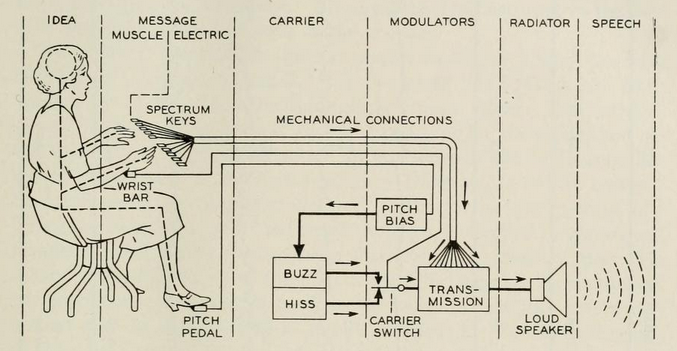
\includegraphics[width=\textwidth]{imagenes/Voder.png}
	\caption{Un esquema del \textit{Voder}. Extraído de \cite{voder}}
\end{figure}

La primera aplicación del reconocimiento de voz fue presentado por IBM en 1962. Con el nombre de \textit{Shoebox}, era una calculadora capaz de reconocer 16 comandos (los dígitos, \textsc{Plus}, \textsc{Minus}, \textsc{Subtotal}, \textsc{Total}, \textsc{False} y \textsc{Off}). Su salida se emitía sin embargo en una impresora.

En 1961, el Doctor J.L Kelly usó un IBM 704 para sintetizar voz a través de un ordenador, cantando una canción en compañía de una orquesta. A partir de ese punto se ha ido trabajando en alas de una voz más natural que se pudiera lanzar con altavoces más pequeños.

En 1972, en el DARPA, se culminó un sistema más complejo de Reconocimiento de Voz denominado \textit{Harpy}, el cual permitía reconocer 1000 palabras e incluso sus combinaciones con tal de crear oraciones y sentencias.

En los 90, se empezó a vender programas software como \textit{Dragon Dictate}, que permitía reconocer bastantes palabras y que se distribuía de forma comercial al público, aunque el monto a gastar por entonces era de 6000 dólares.

\subsubsection{Los primeros Asistentes Virtuales: el don artificial del habla}

El campo de los Asistentes Virtuales ha sido basado en texto durante bastante tiempo, donde a través de un globo podías leer sugerencias y consejos (como ejemplo podemos poner a Clippy, incorporado en 	Microsoft Office 97). Pero hubo dos grandes eventos que dieron pie a la actualidad de los Asistentes de Voz, solapando la los años más recientes. En general, la década de los 2010 ha sido la que estamos continuando actualmente.

\begin{itemize}
	\item Por una parte, el equipo \textit{DeepQA} de IBM se dedicó desde 2004 a hacer un sistema que pudiera responder cualquier pregunta hablada. Este fue más conocido por ganar en simulacros de \textit{Jeopardy} contra campeones de ese programa en 2010 y 2011.
	\item Por la otra, la popularización de los \textit{smartphones} con los iPhone de Apple y la compra de Siri para su posterior mejora, dio la popularidad de los Asistentes Virtuales de Voz que conocemos actualmente.
\end{itemize}

\subsection{En la actualidad...}
Esta era es el apogeo de los Asistentes Virtuales, que están empezando a desarrollarse en multitud de formatos por parte de varias compañías conocidas. En esta parte hablaremos de algunos de ellos a modo introductorio, aunque en el Análisis hablaremos en detalle y analizaremos competitivamente sus habilidades.

\subsubsection {Aplicaciones populares}
Hoy en día, las empresas más importantes tienen una instancia de Asistente Virtual por voz. Comentemos algunas de ellas:

\begin{itemize}
	\item \textbf{Apple Siri} Como se comentó previamente, fue el resultado de la compra de esa aplicación, la cual se integró en el iPhone 4S para darle distintivo a sus dispositivos, presentándose el 14 de Abril de 2011. Con el tiempo se fue extendiendo a los aparatos de Apple, formando parte de su ecosistema.
	\item \textbf{Google Now} Al principio fue diseñado como un sistema de tarjetas que iba aprendiendo de las búsquedas e información del usuario para dar información relevante, pero este no respondía con voz. Posteriormente evolucionó a \textbf{Google Assistant} en Mayo de 2016, primero como parte de una app y extendiéndose de forma análoga a Siri en los dispositivos del ecosistema de Google y Android, siendo este software el que lo enmarca en esta lista.
	\item \textbf{Amazon Alexa} Alexa fue presentada en Noviembre de 2014 para dispositivos Echo. Debido a la gran infraestructura que posee esta multinacional en cuanto a servidores y servicios de \textit{cloud} se refiere, gran parte de ese procesamiento pasa por esas infraestructuras. Además permite hacer aplicaciones (o \textbf{skills}) para que terceros puedan integrarse con este Asistente. Actualmente ha sido integrado en multitud de dispositivos incluso fuera de su ecosistema.También se está ofreciendo como un \textit{SaaS} (\textit{Software as a Service}) para poder integrarlo donde se pueda, además de ciertos plus como voces de famosos.
	\item \textbf{Microsoft Cortana} La respuesta por parte de la empresa de Bill Gates ante el boom del tema a discutir, y tomando la inspiración de una de los personajes más icónicos de \textit{Halo} (uno de los juegos más famosos de la consola de la compañía, \textit{Xbox}), fue presentada en una conferencia de la empresa en Septiembre de 2014. Con la llegada de Windows 10, este asistente llegó integrado. Hay constancia de dos versiones para Android y iOS, pero sólo en inglés.
\end{itemize}

Además de estos, hay un montón más de ellos. En algunos casos, se crean por la falta de soporte de alguno de las empresas más grandes (por ejemplo, \textbf{Huawei Celia} fue desarrollado por las restricciones de Estados Unidos). En otros, por tener otras alternativas con filosofías como el \textit{FOSS}, del cual hablaremos posteriormente. Un ejemplo de ello es \textbf{MyCroft}


\subsubsection{Un sinfín de formatos}
Hoy en día, podemos encontrarnos estas aplicaciones casi en cualquier lado. Si bien en un principio estaba pensado para smartphones, enseguida fue adaptado a otros aparatos.
Una de las propuestas fue con Amazon y su asistente Alexa, que fue embebida en un dispositivo sin pantalla llamado Echo. Sólo dispone de altavoces, micrófonos, una luz para saber si escucha y se podía conectar con el teléfono para poder insertar las contraseñas pertinentes. Posteriormente se hizo una versión que tenía una pantalla para mostrar algunas cosas.
Gracias a la variedad de versiones de ese producto, se permite tener uno de esos Asistentes por precios más o menos caros, con calidades más o menos Premium.

En general, los movimientos en estas aplicaciones tienden a comenzar en un pequeño sector el cual trata de expandirse para formar parte de la experiencia de un ecosistema donde se ha desarrollado.

\begin{figure}[p]
	\centering
	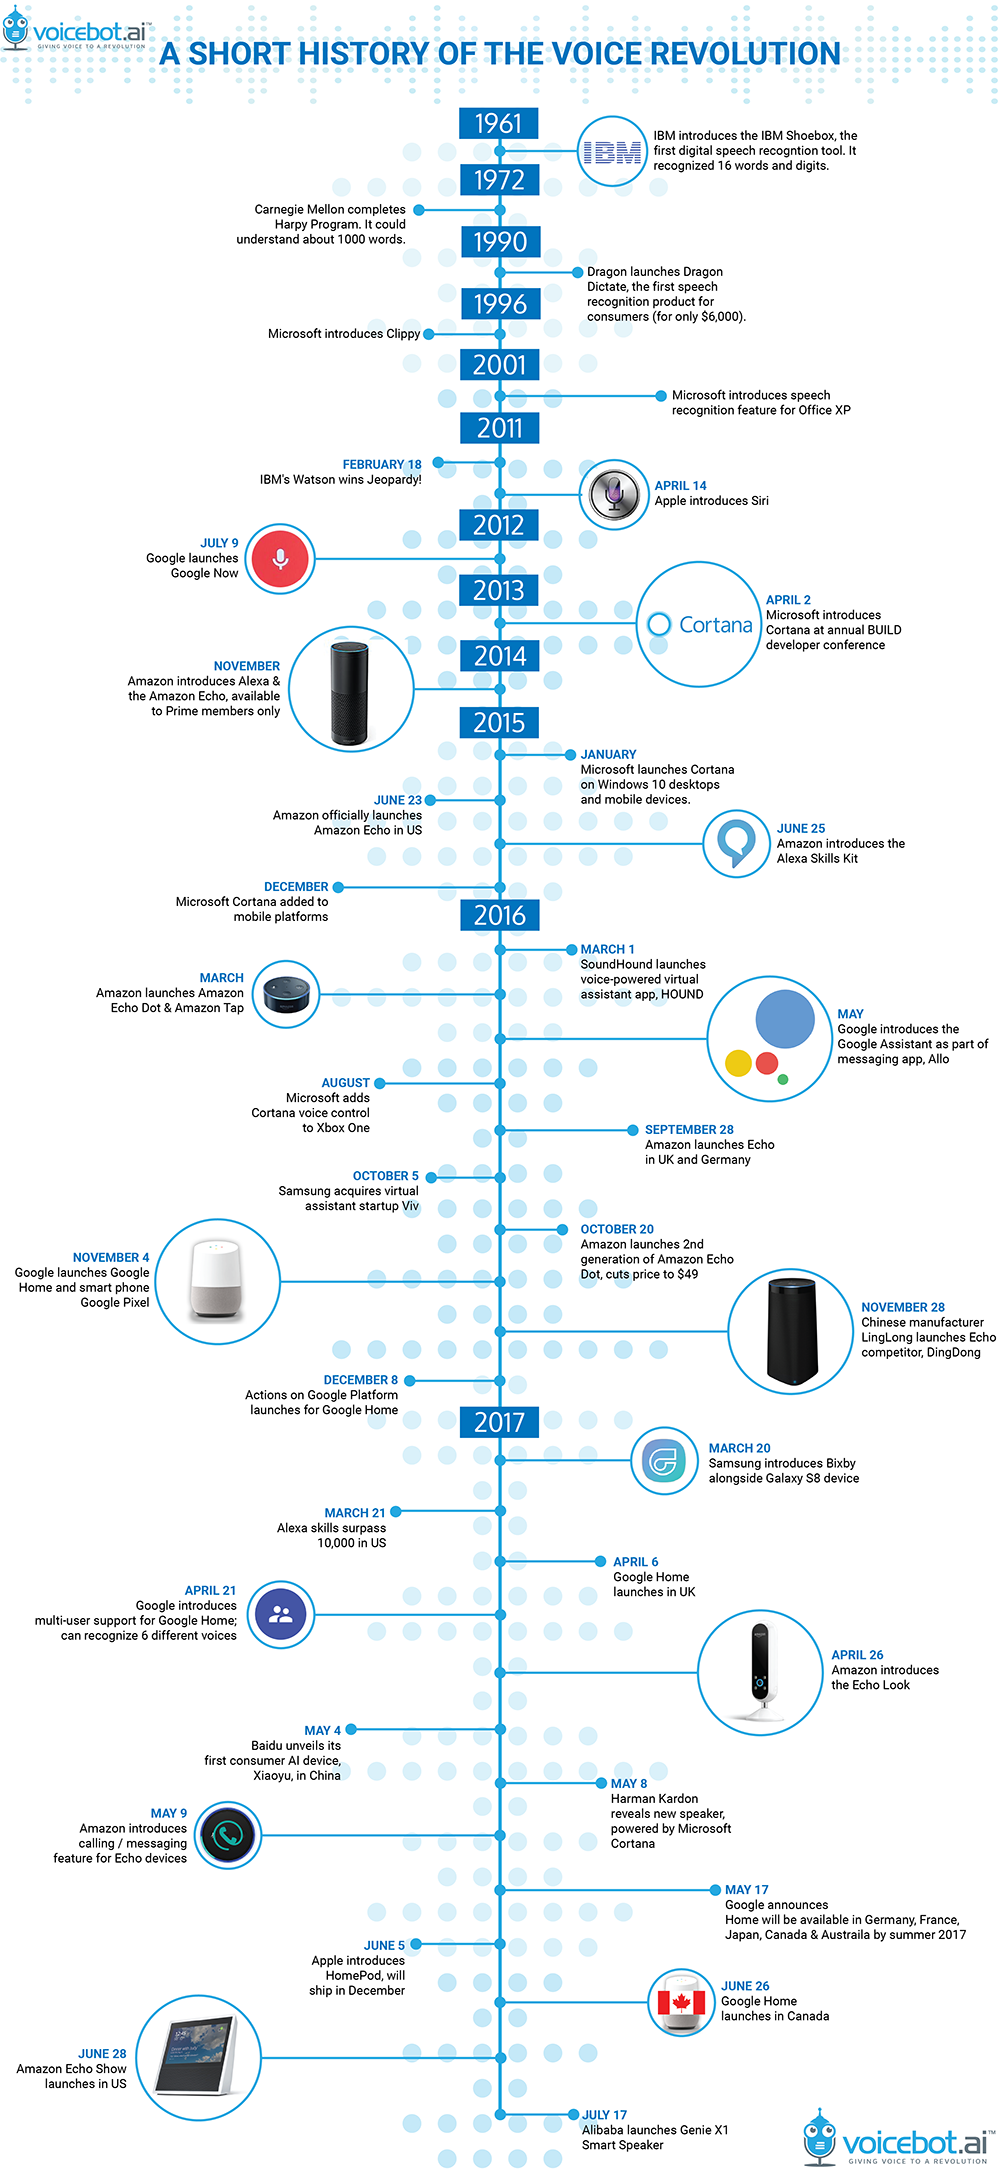
\includegraphics[height=0.98\textheight]{imagenes/Timeline_VA.png}
	\caption{Una timeline con algunos de los eventos más importantes en el área. Extraído de \cite{va-history}}
\end{figure}

\subsubsection{Las ventajas}
 \begin{itemize}
 	\item Una de las más notorias, como hemos visto, es que podemos tener uno de ellos en cualquier sitio. Como hemos comentado antes, desde dispositivos dedicados como los altavoces inteligentes, pasando por ordenadores y \textit{smartphones}, hasta aparatos del Internet de las cosas como \textit{Smart TVs}.
 	\item La información se está solicitando y recibiendo usando la voz, por lo que no es necesario usar las manos o la vista (como hemos comentado en la Introducción), por lo que uno de los usos sería para personas ciegas o con diversidad motora (véase, por ejemplo, la cuadriplejía). Pero además es un punto de acceso para aquella gente que tampoco sepa o pueda leer o escribir, gracias a cómo se puede comunicar la información.
 \end{itemize}
\subsubsection{Las desventajas}
	\begin{itemize}
		\item La más importante está relacionado con la seguridad y privacidad de lo que se usa en ello. Matthew Hoy \cite{vaintroduction-matthewhoy} comentaba en su Introducción a los Asistentes Virtuales que se podría preguntar al propio asistente por información de aquellas cuentas e integraciones que tenga conectadas, o pedirle que le haga tareas.
		
		Como adición a ese comentario, decir algunas de ellas no reconocen exactamente de quién es la voz, por lo que sintetizar la voz para un comando o tener el altavoz de algún dispositivo cerca de este e invocar al software durante una llamada podría ser suficiente para que el Asistente funcione y ejecute lo que se quiera.
		
		Como extra, tengamos en cuenta que uno de los componentes principales de un Asistente de Voz es un micrófono. Aunque conceptualmente sólo sirva para cuando se le llama explícitamente, este igualmente está grabando mientras espera a que se diga su palabra de invocación (o \textit{trigger word}). Como consecuencia, puede generar cierto alarmismo por ese hecho y, en el caso de que alguien pudiera lograr usar ese micrófono para obtener las grabaciones con otros propósitos, generar una brecha de privacidad que podría ser explotada.
		
		\item Si bien se han hecho progresos en los campos del \textit{Speech Recognition} y el \textit{Text-To-Speech}, no son perfectos. Por lo tanto, es posible que ante una petición el comportamiento puede ser un poco indeterminado según la tolerancia del Reconocedor, su entrenamiento y cómo el usuario se exprese.
		
		Por otra parte, la voz que se sintetiza puede llegar a resultar algo robótica, aunque se tratan de hacer esfuerzos en que se intente ser más natural. La otra opción, si se quisiera ser totalmente natural, sería que alguien grabara las voces y estas se reproduzcan, pero además de resultar algo tedioso ya que pueden haber muchas respuestas por grabar, ocupan mucho espacio, algo no muy deseable.
	\end{itemize}

\section{Fundamentos de los Asistentes de Voz}
Por lo analizado a través de la historia y la situación actual podemos intentar extraer un marco teórico que recogería todos los elementos de los Asistentes de Voz y cómo se combinarían para formar algo.

\subsection{Una idea intuitiva}
Para empezar, podríamos empezar con lo que haría un \textit{software} convencional. Se alimenta con una serie de datos, se procesa y acaba saliendo otra serie de datos. Si representáramos ese concepto en un diagrama, tendríamos lo siguiente:

\begin{figure}[H]
	\centering
	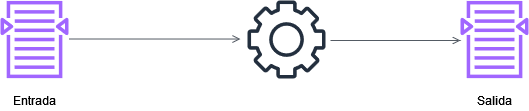
\includegraphics[width=\textwidth]{imagenes/DiagramaBase.png}
	\caption{Diagrama básico de un software}
\end{figure}

Los datos que recoge, en nuestro caso, son voces. Por el otro extremo, lo mismo. Podríamos actualizar nuestro diagrama con esa salida.

\begin{figure}[H]
	\centering
	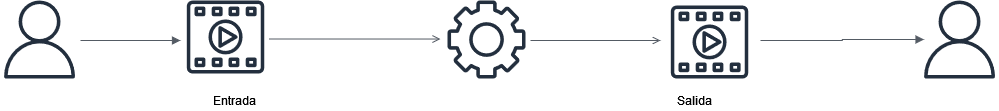
\includegraphics[width=1.1\textwidth]{imagenes/DiagramaDatos.png}
	\caption[Diagrama modificado.]{Diagrama modificado. Nótese que en vez de documentos se usa multimedia}
\end{figure}

Esas voces que se recogen no se generan solas. En el caso de la recogida, es un usuario quien habla a través de un micrófono para grabar esa voz que podrá procesar posteriormente. En el otro lado, esa voz se reproducirá a un altavoz. Esos procesos de grabación y reproducción tienen ya de por si su propia lógica intermedia para poder procesarlos. Con esta nueva información, el diagrama quedaría de la siguiente forma:

\begin{figure}[H]
	\centering
	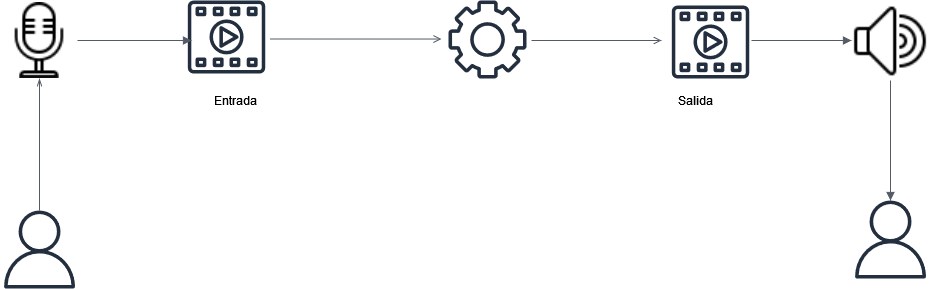
\includegraphics[width=1.1\textwidth]{imagenes/DiagramaIO.png}
	\caption[Diagrama con E/S.]{El mismo diagrama que el anterior, pero señalando las Entradas y Salidas.}
\end{figure}

Ahora tenemos otras dos cuestiones sobre esos archivos de audio.
\begin{itemize}
	\item ¿Cómo puede entender \textbf{qué está diciendo esa voz}?
	\item ¿Cómo se crea \textbf{el audio de la respuesta} a partir de un texto?
\end{itemize}
La respuesta a esas dos preguntas resulta ir en dos campos respectivos de la Inteligencia Artificial: el \textbf{Reconocimiento} (o \textit{\textbf{Speech Recognition}}) y la \textbf{Síntesis de Voz} (conocido más como \textbf{\textit{Text-to-Speech}}). 

Por lo tanto, se crea una lógica para poder hacer esas conversiones, de forma que podríamos hacer que el sistema nos escriba qué ha entendido (reconociendo esa voz) y que ``lea'' la respuesta con lo que le hayamos escrito (sintetizando la voz). De todas maneras, hablaremos de ello más adelante. Podríamos actualizar el diagrama resultando en esta figura.

\begin{figure}[H]
	\centering
	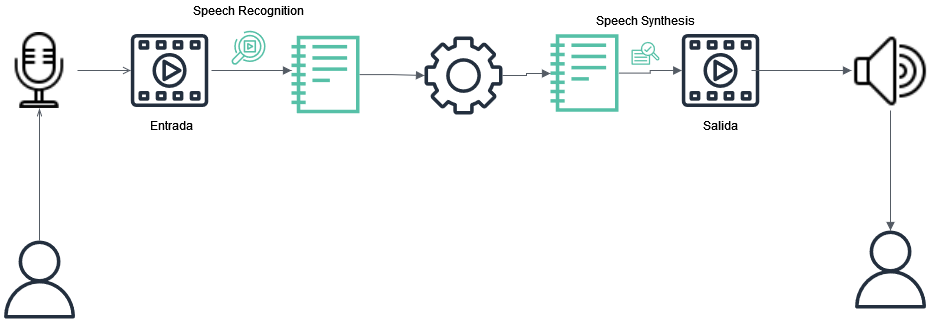
\includegraphics[width=1.1\textwidth]{imagenes/DiagramaTTS_SR.png}
	\caption[Diagrama con TTS/SR]{El diagrama anterior pero señalando las interacciones con el Speech Recognition y el Text-To-Speech (o Speech Synthesis)}
\end{figure}

Por último, la lógica que hay entre lo que se ha dicho y lo que tiene que leer la máquina debería poder procesar esa frase, buscar si sigue algún patrón o usa alguna palabra de relevancia (como ``Reproduce'', ``Canta'' o ``El tiempo en una ciudad''), y dar una respuesta que se pueda leer. Por lo tanto, el diagrama final a modo conceptual podría darse como la de la siguiente figura: 

\begin{figure}[H]
	\centering
	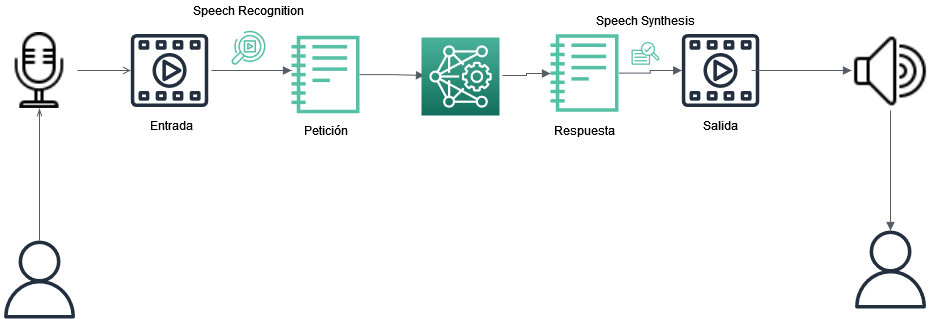
\includegraphics[width=1.1\textwidth]{imagenes/DiagramaIntuitivo.png}
	\caption[Diagrama intuitivo final.]{Diagrama resultante. Nótese que la lógica en verdad es un proceso de relacionar conceptos.}
\end{figure}

En resumen, podríamos decir que un Asistente de Voz consta a nivel \textit{hardware} de un ordenador con un micrófono o entrada de audio y un altavoz o salida de audio.

Sin embargo, a nivel \textit{software} necesitaríamos:
\begin{enumerate}
	\item Un módulo para gestionar las \textbf{grabaciones del micrófono} que diga cuándo grabar, cuando parar, y que guarde la grabación para poder trabajar con esta. Esta nos devuelve un audio
	\item Una parte para hacer \textbf{Reconocimiento de Voz} a través de esa grabación. Nos devuelve el mensaje de ese audio.
	\item La \textbf{lógica principal} del programa, que mira el mensaje y responde con otro.
	\item Una parte para poder hacer \textbf{Text-To-Speech}, convirtiendo la respuesta en otro audio.
	\item Un módulo para poder \textbf{reproducir ese audio} con la respuesta a través del altavoz, que cargue el archivo y lo reproduzca.
\end{enumerate}

\subsection{El reconocimiento de voz}
En la documentación sobre el tema, IBM \cite{sr-definition} define el Reconocimiento de Voz o \textit{Automatic Speech Recognition} (ASR) como la capacidad de un programa de procesar el habla y convertirlo en un texto escrito legible, que puedan entender también las máquinas para el posterior procesado de la información.


\subsection{La síntesis de voz}

\subsection{La lógica}

\section{Software Libre, Software de Código Abierto y Licencias}
El software libre y sus licencias \cite{gplv3} ha permitido llevar a cabo una expansión del
aprendizaje de la informática sin precedentes.
\subsection{¿Desde cuándo existe?}

\subsection{¿En qué beneficia liberar el código?}

\subsection{El curioso mundillo de las Licencias y sus restricciones}

\subsubsection{Detallando el marco legal de las Licencias}

\subsubsection{Free Software Foundation}

\subsubsection{Creative Commons}

\subsubsection{Otros tipos de licencias}

\subsubsection{¿Puedo crear una licencia?}
